\documentclass[10pt,a4paper]{article}
\usepackage{graphicx}
\usepackage{amssymb}
\usepackage{fullpage}
\usepackage{amsmath}

\title{Senior Quantum 2011 Assignment 2}
\date{}
\author{D. G. Wilcox \\
		309248035}

\begin{document}
\maketitle
\section*{Question 1}
\begin{itemize}
	\item[(a)] If $A$ is the atomic transition rate from the excited state to the ground state, the population of the excited state $N$ is described by the equation:
		\begin{equation*}
			\frac{dN}{dt} = - A N
		\end{equation*}
	which we can solve to get:
		\begin{align*}
			N(t) &= N_{0}e^{-At} \\
			\Rightarrow \tau &= \frac{1}{A} \\
		\end{align*}
	
	\item[(b)] The rate of transition is $A$, therefore $\Delta t = \tau$, giving:
		\begin{align*}
			\Delta E &\geq \frac{\hbar}{2 \Delta t} \\
			&\geq 3.94 \times 10^{-27} \\
		\end{align*}
	where $\Delta E$ is measured in Joules.

	\item[(c)] We can find a relation between $\Delta \lambda$ and $\Delta E$ via the following:
		\begin{align*}
			E &= \frac{hc}{\lambda} \\
			\Delta E &= E_{1} - E_{2} = hc [\frac{1}{\lambda_{1}} - \frac{1}{\lambda_{2}}] \\
			&= hc [\frac{\lambda_{2} - \lambda_{1}}{\lambda_{1}\lambda_{2}}] \\
			&= hc [\frac{\Delta \lambda}{\lambda^{2}}] \\
			\Rightarrow \Delta \lambda &= \Delta E \frac{\lambda^{2}}{hc} \\
			&= 4.02 \times 10^{-15} \\
		\end{align*}
	where $\Delta \lambda$ is in metres.

	\item[(d)] A forbidden transition has a much smaller transition probability. This means $\Delta t$ is larger and so $\Delta E$ is smaller.
\end{itemize}

\section*{Question 2}
\begin{itemize}
	\item[(a)] The selection rules $\Delta j = 0, \pm 1$, $\Delta l = \pm 1$,
		\begin{align*}
			^{2}P_{3/2} &\rightarrow ^{2}S_{1/2} &: \Delta j = 1, \Delta l = 1  \\
			^{2}P_{1/2} &\rightarrow ^{2}S_{1/2} &: \Delta j = 0, \Delta l = 1  \\
			\therefore &\mbox{ Both transitions are allowed}& \\
		\end{align*}
	
	\item[(b)] 
		\begin{figure}[!h]
			\begin{center}
				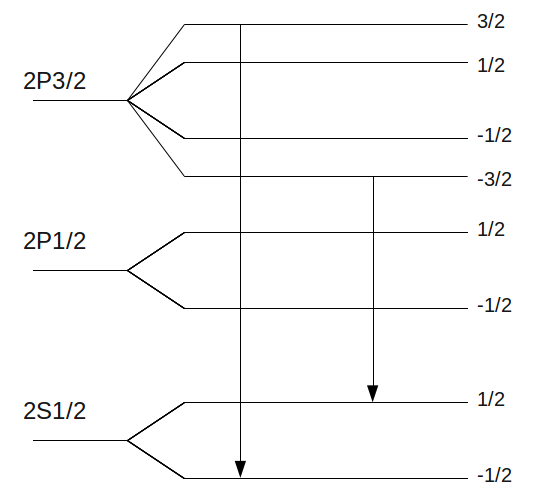
\includegraphics[width=0.8\linewidth]{energyLevels.png}
			\end{center}
			\caption{Energy Level Diagram. Forbidden transitions are labeled with arrows.}
		\end{figure}

	\item[(c)] The selection rules for magnetic angular momentum $m_{j} = 0, \pm 1$.

	\item[(d)] The Land\' e $g$-factor is given by the equation:
		\begin{equation*}
			g = 1 + \frac{j(j+1)+s(s+1)-l(l+1)}{2j(j+1)}
		\end{equation*}
	
	Giving $^{2}P_{3/2} \rightarrow 4/3$ and $^{2}P_{1/2} \rightarrow 5/2$.

	\item[(e)] The value of the magnetic field is found by equating the two energies with their energy changes:
		\begin{align*}
			E_{1} + \Delta E_{1} &= E_{2} + \Delta E_{2} \\
			B = \frac{E_{2} - E_{1}}{k_{1}-k_{2}} \\
		\end{align*}
	where $\Delta E = \mu_{b}B m_{j}g$ and $k_{n} = \mu_{b}m_{n}g$. Using $E = \frac{hc}{\lambda}$ we get:
		\begin{equation*}
			B = 15.87 \mbox{ T}
		\end{equation*}
\end{itemize}

\section*{Question 3}
\begin{itemize}
	\item[(a)] Using:
		\begin{align*}
			E_{r} &= \frac{\hbar^{2}}{2I}r(r+1) &\\
			E_{r} - E_{r+1} &= -\frac{\hbar}{I}(r+1) &, r = 0,1,2,.. \\
		\end{align*}
		which increases linearly with r.
	
	\item[(b)] Subbing into the equation derived above:
		\begin{align*}
			E_{r} &= \frac{\hbar^{2}}{2I}r(r+1) \\
			\Rightarrow 0.106 &= \frac{\hbar^{2}}{2\mu R_{0}^{2}} \\
			R_{0} &= \frac{-\hbar}{\sqrt{(\mu \times 0.106}} \\
					  &= -7.99 \times 10^{-21} \\
		\end{align*}
	where $R_{0}$ is measured in metres.

	\item[(c)] By treating the molecule as a rigid motor we are simplifying our model. Realistically, as the rotational energy increases the bond distance will increase.
\end{itemize}
\section*{Question 4}
\begin{itemize}
	\item[(a)] 
		\begin{figure}[!h]
			\begin{center}
				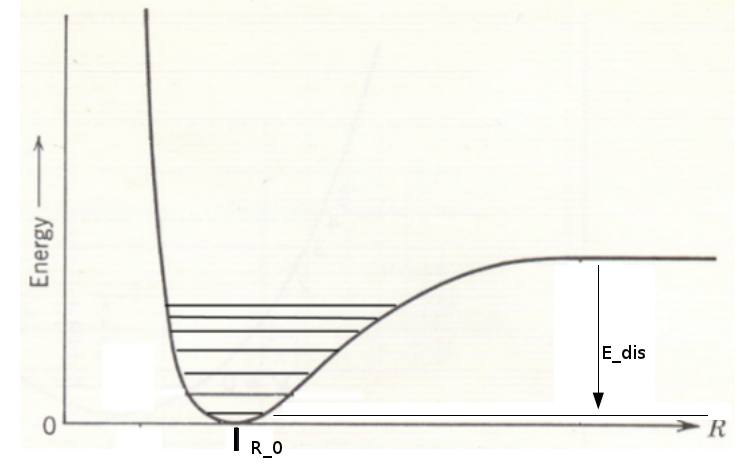
\includegraphics[width=0.8\linewidth]{potentialCurve.png}
			\end{center}
			\caption{Potential Curve Diagram.}
		\end{figure}

	\item[(b)] The lowest vibrational state occurs at $v = 0$:
		\begin{align*}
			E_{v} &= \frac{1}{2}h \nu_{0} \\
			      &= 2.78 \times 10^{-20} \\
		\end{align*}

	\item[(c)] The vibrational levels will have an even spacing between them when the potential curve is a parabola, which is the case for lower vibrational levels. As the energy increases the curve becomes less like a parabola and the spacings cease to be regular.

	\item[(d)] When the molecule transitions between different states there are "transitions upon transitions". This is what causes the series of bands of spectral lines.
\end{itemize}
\end{document}
